\documentclass[journal]{IEEEtran}
\usepackage{amsmath,amssymb,booktabs,cite,graphicx,placeins}
\usepackage[hidelinks]{hyperref}
\begin{document}
\raggedbottom
\title{Ranking and Allocation of Boundary Edits for SAR Ship Instance Segmentation}
\author{Author~Details~Pending\thanks{Review version. Author affiliations and corresponding-author details are pending.}}
\maketitle

\begin{abstract}
A one-pixel displacement can substantially reduce the overlap of a narrow ship mask in synthetic aperture radar (SAR) imagery. We estimate occupancy on the native detector grid and refine retained masks at a controlled edit count. On HRSID DEV705, at fixed addition and removal counts, optimizing pairs within the original displacement cap adds 0.48 mask average precision (AP) points, and independent ranking adds a further 0.43. On the 74-chip Instance-RSDD reserve, independent ranking exceeds bounded re-pairing by 0.48 AP. Relative to distance-first pairing, one-pixel boundary IoU gains 0.47 points for one Gaofen-3 detector fit and 0.70 points on the reserve. The second fit's interval includes zero. In a separate comparison with a fixed total edit count, varying the addition--removal split improves AP by 2.30 and 1.75 points under two SSDD references across three head fits. The frozen SAR-SSP transfer loses 0.14 AP points.
\end{abstract}

\begin{IEEEkeywords}
Synthetic aperture radar, ship instance segmentation, boundary refinement, native image grid.
\end{IEEEkeywords}

\section{Introduction}
\label{sec:introduction}

A detector may localize a ship correctly while its mask follows a neighboring quay or cuts across the bow. The error matters on a thin hull. Translating a \(w\)-pixel-wide rectangle by one pixel across its short axis preserves its area but changes its intersection over union (IoU) to \((w-1)/(w+1)\), or \(0.60\) at \(w=4\). Close to shore, a nearby bright return can further complicate the decision about which foreground cells belong to the ship~\cite{hrsid,rsdd,gao2024}.

A reference-guided analysis of retained HRSID masks motivates editing both sides of the contour. Among 1,329 matched instances with area below 1,024 pixels and aspect ratio at least two, expanding the detection box by two pixels permits 134 more instances to attain continuous IoU of 0.90. Expanding the foreground only within the new strip reaches this threshold in zero of those cases. At least 91 require additions and removals inside the original box. These reference-guided ceilings motivate separate tests of where to edit and how much area to change.

We study these decisions on the native detector grid. We first fix the numbers of additions and removals separately. A distance-paired editor may have to remove a good foreground cell to make a useful addition nearby. Independent rankings release this coupling while keeping both counts, the scores, and the candidate identities fixed. We then hold the total number of changes fixed and vary the split, which allows changes in the predicted area. Our contributions are as follows.
\begin{enumerate}
\item We train a lightweight occupancy head with fractional polygon--cell coverage. The same features and native geometry support candidates from D-FINE-seg and RF-DETR~\cite{dfine,rfdetr}.
\item At the same realized signed counts, we compare distance-first pairing, gain-maximizing pairing with the original displacement cap, and independent endpoint ranking. Frozen experiments measure how location choices affect AP and continuous overlap on author-labeled cohorts, with a separate assessment at native boundary scales.
\item We use a second, two-output occupancy head to test signed allocation at a fixed total. The controlled comparisons retain the estimated-IoU objective while varying the available splits. Two SSDD reference releases, a frozen transfer test, and pretrained-refiner controls quantify the gains and the limits of changing area and writable support.
\end{enumerate}

\section{Related Work}
\label{sec:related-work}

\textit{SAR ship masks.} HRSID, the polygon subset of SSDD, and Instance-RSDD enable assessment of individual hulls from SAR images~\cite{hrsid,ssdd,rsdd}. Rotated regions and dual-scale attention align features with the long axis~\cite{rsdd,drsnet}. Dynamic scattering key points and geometry-aware feature fusion help generate masks in cluttered scenes~\cite{gao2024,dacf,gcie}. GLDet mines local gradients upstream of detection~\cite{gldet}. DSR-Net evolves a contour inside a region of interest using physical-gradient and curvature terms~\cite{dsr}. SISS-YOLO uses coordinate attention and an IoU-weighted loss for multiclass Sentinel-1 ship instances~\cite{siss}. Given a retained mask and score, we use fractional occupancy to isolate decisions about boundary edits on the detector grid.

\textit{Signed updates and overlap.} Spatial-attraction mapping exchanges labels to preserve the foreground proportion~\cite{atkinson,xu}. RankSEG uses posterior ranking and foreground volume selection for overlap objectives~\cite{rankseg}. Its reciprocal-moment and local-dependence variants address expected overlap under different probability assumptions~\cite{rankrma,rankdep}. In our setting the original mask fixes the two types of eligible sites. The detector score, candidate, support and per-candidate budget provide a common comparison for the effect of the pairing constraint and for the effect of signed allocation.

\textit{Mask refinement.} PointRend samples uncertain positions during subdivision, SegFix corrects boundary labels using interior estimates, and boundary patch refinement predicts updates in image and mask patches~\cite{pointrend,segfix,bpr}. RefineMask incorporates progressively finer features~\cite{refinemask}. Phoenix and SegRefiner revise an input coarse mask~\cite{phoenix,segrefiner}. A whole-mask output combines the estimated response with the rule for writing it. Holding a response fixed while changing writable support or the edit count lets us distinguish the consequences of these two choices.

\section{Method}
\label{sec:method}

\subsection{Overview}
A frozen detector supplies a mask \(M\), box \(B\), confidence \(s\), and decoder response \(p_i\) sampled on native image cell \(i\). We estimate occupancy on both sides of the contour (Section~\ref{sec:occupancy}), then test pairing at fixed signed counts (Section~\ref{sec:selection}) and allocation at fixed total count (Section~\ref{sec:variable-sign}). Detection identities, classes, boxes, and scores are fixed. A parallel control changes the write rule on one frozen Phoenix response (Fig.~\ref{fig:native-boundary}).

\begin{figure*}[!t]
\centering
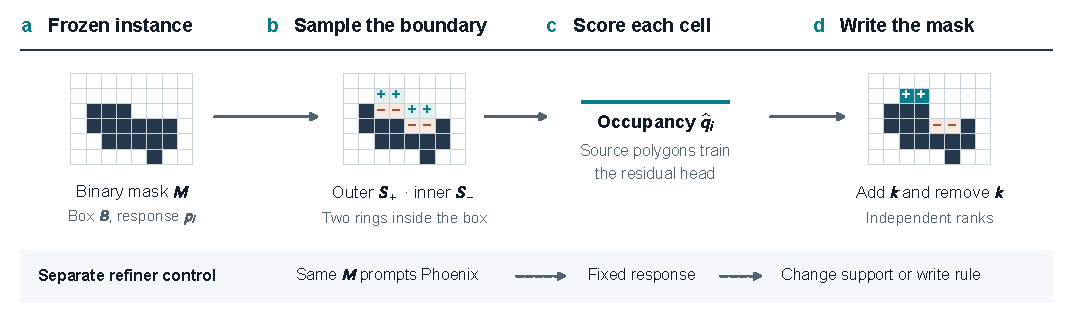
\includegraphics[width=\textwidth]{figures/matched_budget_pipeline.pdf}
\caption{The local pipeline fixes the detector output, samples native boundary cells, estimates their occupancy, and writes the selected edits. The lower lane compares writing rules on the same frozen refiner response.}
\label{fig:native-boundary}
\end{figure*}

\subsection{Native-Grid Sampling and Occupancy}
\label{sec:occupancy}
Let \(\Omega\) be the decoded \(W\)-by-\(H\) grid. Cell \(i=(x,y)\) covers \(C_i=[x,x+1)\times[y,y+1)\), and \(M_i=\mathbf{1}\{i\in M\}\). For \(B=[x_1,x_2)\times[y_1,y_2)\), inclusion is tested on the integer indices \(x,y\). For a response plane of width \(W_m\), native column \(x\) maps to \((x+\tfrac12)W_m/W-\tfrac12\), with the corresponding height map. D-FINE supplies a \(160\times160\) uncropped sigmoid plane. Its CPU feature path rounds the plane to FP16, bilinearly interpolates in FP32 with edge clamping, and rounds the sample to FP16. RF-DETR applies sigmoid after interpolating its logits. The saved binary mask determines the edit sign, including at sites where the sampled response and native binary decision differ.

For \(32\le |M|<1024\), use square \(3\times3\) dilation \(\delta\) and erosion \(\varepsilon\) with zero exterior. The two-layer support pools are
\begin{equation}
\begin{aligned}
\mathcal B_+&=(\delta^2(M)\setminus M)\cap B\cap\Omega,\\
\mathcal B_-&=(M\setminus\varepsilon^2(M))\cap B\cap\Omega.
\end{aligned}
\label{eq:native-bands}
\end{equation}
Layer \(\ell_i\) is one in the first ring and two in the second. We retain the first \(n=\min(32,|\mathcal B_+|,|\mathcal B_-|)\) sites on each side in ascending order of \((|p_i-\tfrac12|,yW+x)\), giving \(S_+\) and \(S_-\). Masks outside the area range or with \(n=0\) retain their original shape. Fig.~\ref{fig:occupancy-stage} shows the native support and supervision.

\begin{figure}[t]
\centering
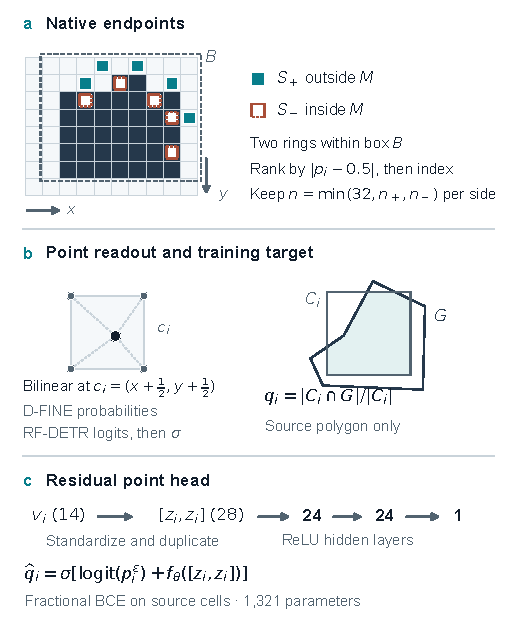
\includegraphics[width=\columnwidth]{figures/method_native_occupancy.pdf}
\caption{The two native rings supply candidate additions and removals. The reference polygon supplies fractional cell coverage during training, and the point head corrects the decoder response with a learned logit residual.}
\label{fig:occupancy-stage}
\end{figure}

A source-training candidate supplies supervision if it has a nonignored native COCO match at the raster IoU threshold of \(0.50\) and a valid reference polygon \(G\). Its target is the area fraction
\begin{equation}
q_i=|C_i\cap G|/|C_i| .
\label{eq:fractional-target}
\end{equation}
The 14 inputs comprise response and membership, boundary geometry, box-relative and candidate descriptors, and local appearance. In implementation order, the vector is
\begin{equation}
\begin{aligned}
v_i=\big(&p_i,M_i,\ell_i,d_i,\bar x_i,\bar y_i,\nu,\eta,s,\\
        &L_i,\bar L_3(i),\bar L_5(i),\Delta_x L_i,\Delta_y L_i\big)^\top .
\end{aligned}
\label{eq:endpoint-features}
\end{equation}
Here \(d_i\) is Euclidean distance to the nearest opposite-class cell, with background outside the grid. The box coordinates are \(\bar x_i=(x-x_1)/(x_2-x_1)\) and \(\bar y_i=(y-y_1)/(y_2-y_1)\). Area descriptors are \(\nu=\log_2|M|\) and \(\eta=|M|/|B\cap\Omega|\), with the latter denominator counting native box indices. The decoded red, green, and blue values \(c_i^R,c_i^G,c_i^B\) give \(L_i=(0.299c_i^R+0.587c_i^G+0.114c_i^B)/255\). With edge replication, the local mean and horizontal difference are
\begin{equation}
\begin{aligned}
\bar L_w(i)&=w^{-2}\!\!\sum_{j\in\mathcal N_w(i)}L_j,\\
\Delta_x L_i&=(L_{x+1,y}-L_{x-1,y})/2 ,
\end{aligned}
\label{eq:appearance-features}
\end{equation}
where \(\mathcal N_w(i)\) is the centered \(w\times w\) neighborhood and \(\Delta_y L_i\) uses the analogous row difference.

In the single-reference head, \(E_j\) averages training endpoints in source group \(j\). The training-only standardization uses
\begin{equation}
\mu=J^{-1}\sum_{j=1}^{J}E_j[v],\quad
\sigma_v^2=J^{-1}\sum_{j=1}^{J}E_j[v^2]-\mu^2 .
\label{eq:group-standardization}
\end{equation}
We clip negative roundoff in the variance to zero and use unit scale when the resulting scale is below \(10^{-12}\). For \(z_i=(v_i-\mu)/\sigma_v\) and \(p_i^\epsilon=\operatorname{clip}(p_i,10^{-4},1-10^{-4})\), the prediction is
\begin{equation}
\widehat q_i=\operatorname{sigmoid}
 \big(\operatorname{logit}(p_i^\epsilon)+f_\theta([z_i,z_i])\big).
\label{eq:occupancy-head}
\end{equation}
The two-hidden-layer ReLU head maps \(28\to24\to24\to1\) with 1,321 parameters. Input duplication matches the capacity of the partner-context control. The final affine layer starts at zero, so initial predictions follow the clipped response. Each batch samples groups uniformly and takes a pair within each sampled group. With \(m=64\), the loss averages both sides.
\begin{equation}
\mathcal L_{\rm occ}=\frac{1}{2m}\sum_{j=1}^{m}
  \left[\operatorname{BCE}(q_{a_j},\widehat q_{a_j})+
        \operatorname{BCE}(q_{d_j},\widehat q_{d_j})\right].
\label{eq:occ-loss}
\end{equation}
Here \(\operatorname{BCE}(y,p)=-y\log p-(1-y)\log(1-p)\). AdamW runs for 200 updates with learning rate \(0.002\) and weight decay \(0.01\). Each FIT109 development fold excludes its held source prefixes from fitting and standardization. Transfer freezes the weights and scaling obtained from all FIT109.

\subsection{Endpoint Selection at Equal Signed Counts}
\label{sec:selection}
List \(S_+\) and \(S_-\) in row-major order as \(a_j\) and \(d_j\). Fixed pairing first solves
\begin{equation}
\pi^\star\in\arg\min_{\pi\in\mathfrak S_n}
  \sum_{j=1}^n\|a_j-d_{\pi(j)}\|_2^2 .
\label{eq:fixed-assignment}
\end{equation}
We keep the assignment returned by SciPy on this integer cost matrix. The fixed writer ranks the pair gains \(\widehat q_{a_j}-\widehat q_{d_{\pi^\star(j)}}\) in descending order with addition-row ties. It keeps positive gains up to \(K=\min(8,\lfloor |M|/10\rfloor,n)\). Denote the realized count by \(k\), including the case \(k=0\). At this same count the independent writer solves
\begin{equation}
\max_{\substack{A\subseteq S_+,\,D\subseteq S_-\\ |A|=|D|=k}}
  \left(\sum_{i\in A}\widehat q_i-\sum_{i\in D}\widehat q_i\right).
\label{eq:independent-estimated-gain}
\end{equation}
This selects the highest occupancies on the addition side and the lowest on the removal side, breaking ties by the original pairing-row ordinal. The natural-count comparison retains positive gains under the independent ranks up to \(K\). Figure~\ref{fig:selection-stage} illustrates the fixed-count comparison.

The bounded writer tests whether reassigning partners accounts for the gain while preserving the maximum individual displacement. For \(k>0\), let \(H_{\rm fix}\) contain the \(k\) accepted pairs of the distance-first writer. Set \(\rho^2=\max_{(a,d)\in H_{\rm fix}}\|a-d\|_2^2\). On the graph with edges satisfying \(\|a-d\|_2^2\le\rho^2\), the bounded writer solves
\begin{equation}
\max_{\substack{H\ \text{matching}\\ |H|=k}}
\sum_{(a,d)\in H}(\widehat q_a-\widehat q_d).
\label{eq:bounded-endpoint-matching}
\end{equation}
Each site appears at most once. If the independent endpoint sets admit such a matching, we use them. Otherwise we solve \eqref{eq:bounded-endpoint-matching} by unit-capacity minimum-cost flow. The cap applies to individual edges. Total displacement and connectivity can vary. The three feasible sets are nested, so the estimated gains are ordered from distance-first to bounded to independent.

\begin{figure*}[!t]
\centering
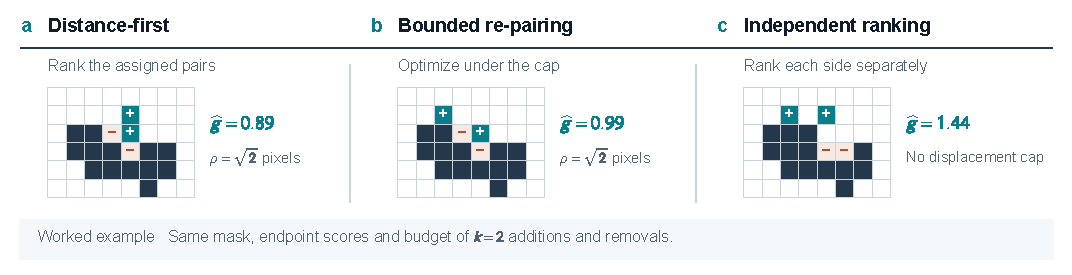
\includegraphics[width=\textwidth]{figures/method_bounded_selection.pdf}
\caption{Three writers at the same signed counts. The bounded writer re-pairs sites under the inherited displacement cap. Independent selection removes this cap. The worked example marks the two additions and removals in each output. The value \(\widehat g\) is the estimated intersection gain.}
\label{fig:selection-stage}
\end{figure*}

Write \(P=|M|\), \(T=|G|\), \(I=|M\cap G|\), and \(U=P+T-I\) in native area units. For the edited mask \(W'=(M\setminus D)\cup A\), its area change \(d\) and exact intersection change \(g\) are
\begin{equation}
d=|A|-|D|,\qquad
g=\sum_{i\in A}q_i-\sum_{i\in D}q_i .
\label{eq:intersect-changes}
\end{equation}
The new mask has area \(P+d\), intersection \(I+g\), and union \(U+d-g\). Subtracting \(I/U\) gives
\begin{equation}
\Delta\mathrm{IoU}=\frac{(P+T)g-Id}{U(U+d-g)} .
\label{eq:variable-area}
\end{equation}
For equal signed counts, \(d=0\) and IoU strictly increases with \(g\). Let \(g_{\rm pair}\) and \(g_{\rm ind}\) be the true gains under distance-first and independent selection. Common edits cancel, leaving the symmetric difference \(\mathcal D\) of the written sites. Optimality under the estimated gains gives
\begin{equation}
g_{\rm pair}-g_{\rm ind}
 \le \sum_{i\in\mathcal D}|\widehat q_i-q_i|
 \le 4k\max_{i\in S_+\cup S_-}|\widehat q_i-q_i| .
\label{eq:selection-error}
\end{equation}
Occupancy errors can reverse the ordering for a fixed match. COCO can also reassign matches at each IoU threshold.

\subsection{Dual-Reference Allocation at a Fixed Total Count}
\label{sec:variable-sign}
For the D-FINE allocation comparison, dynamic attraction supplies the candidate count \(k_s\), and static attraction at that count supplies the incumbent action \(S=(A_S,D_S)\) (Section~\ref{sec:phoenix}). A separate 1,346-parameter head takes the duplicated 14-dimensional feature vector and uses two 24-unit hidden layers. It applies the residual form in \eqref{eq:occupancy-head} with a separate final output for each reference. Training uses binary raster targets from paired author instances with mutual raster IoU at least \(0.50\) and the same native detection match. Eligible candidates have \(n>k_s>0\) and at least one nonidentity action. The 848 qualifying candidates span 447 images in 439 decoded groups. The head uses training-only group, image, candidate, and endpoint weighting for scaling. Each of 1,000 AdamW updates samples 64 candidates through groups and images, using a learning rate of 0.002 and weight decay of 0.01. BCE averages the signed endpoints and both references within a candidate, then weights each sampled candidate equally. At each seed all allocation policies use the same head.

Let \(E=S_+\cup S_-\) and \(\widehat q_{ir}\) denote occupancy under reference \(r\). Outside \(E\) the approximation takes the native labels as deterministic. Thus,
\begin{equation}
\begin{aligned}
\widehat T_r&=|M\setminus E|+\sum_{i\in E}\widehat q_{ir},\\
\widehat I_{r0}&=|M\setminus E|+\sum_{i\in E\cap M}\widehat q_{ir}.
\end{aligned}
\label{eq:dual-area-proxy}
\end{equation}
With \(g_r=\sum_{i\in A}\widehat q_{ir}-\sum_{i\in D}\widehat q_{ir}\) and \(d=|A|-|D|\), the ratio of expected intersection to expected union is
\begin{equation}
\widehat f_r(A,D)=
\frac{\widehat I_{r0}+g_r}{P+d+\widehat T_r-\widehat I_{r0}-g_r}.
\label{eq:dual-est-iou}
\end{equation}
Write \(a=|A|\) and \(b=|D|=2k_s-a\). The feasible integer range is \(\max(0,2k_s-n)\le a\le\min(n,2k_s)\). For \(\lambda\in\{0,0.1,\ldots,1\}\), we rank the two sides by \(\lambda\widehat q_{i1}+(1-\lambda)\widehat q_{i2}\), descending for additions and ascending for removals. Endpoint ties follow the archived order. For each split, we cross the first \(a\) and \(b\) entries of the corresponding side orders across all mixtures and add the incumbent side where its count permits. This gives a finite menu of action pairs, with score
\begin{equation}
J(A,D)=\min_{r\in\{1,2\}}\left[\widehat f_r(A,D)-\widehat f_r(S)\right].
\label{eq:dual-maximin}
\end{equation}
The incumbent is evaluated first. Splits follow increasing \(|a-k_s|\) and then \(a\), with ties retaining the first action. The equal control admits only \(a=k_s\), and a sensitivity admits feasible \(a\in\{k_s-1,k_s,k_s+1\}\). The proposal rule and total \(2k_s\) flips are shared (Fig.~\ref{fig:signed-allocation}). Alternative full-menu objectives use mean IoU gain or minimum raw-intersection gain.

\begin{figure*}[!t]
\centering
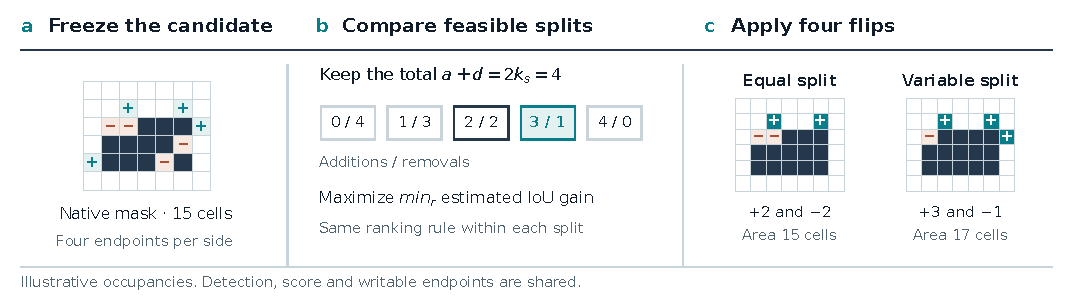
\includegraphics[width=\textwidth]{figures/method_signed_allocation.pdf}
\caption{Illustrative allocation at a fixed total of four flips. The equal split adds two cells and removes two. The maximin choice in this example adds three and removes one, changing the final area at the same total count.}
\label{fig:signed-allocation}
\end{figure*}

Equation~\eqref{eq:dual-est-iou} uses the reciprocal of the mean union, as in the RankIoU approximation~\cite{rankrma}. To assess this approximation on the same menu, we also compute the exact expectation under an independent Bernoulli model for the uncertain cells of each reference. The overlap \(I_r(W')\) and foreground count \(Z_r(W')\) outside \(W'\) involve disjoint sites. Their independence gives
\begin{equation}
\widehat f^{\rm E}_r(W')=\mathbb E[I_r(W')]\,
             \mathbb E[(|W'|+Z_r(W'))^{-1}] .
\label{eq:exact-iou-signed}
\end{equation}
The uncertain part of \(Z_r(W')\) follows the Poisson-binomial law~\cite{rankseg}. Both scores use the same incumbent and deterministic native labels outside \(E\).

\subsection{Controlled Writing of a Frozen Refiner Response}
\label{sec:phoenix}
The decoded image and native mask prompt Phoenix XL1~\cite{phoenix}. We share the same output probabilities \(r_i\) after five refinement iterations across all writers. Writable support \(\mathcal W\) is either the sampled boundary \(E\) or the full grid \(\Omega\). The threshold writer uses the author's selected binary hypothesis in \(\mathcal W\) on the shared positive-budget candidates. The count writer makes exactly \(2k_{\rm att}\) flips, where \(k_{\rm att}\) is obtained from dynamic spatial attraction~\cite{atkinson}. At exchange \(\tau\) the attraction is
\begin{equation}
h_\tau(i)=\sum_{j\in M_\tau}
 e^{-\|i-j\|_2/5}\,\mathbf 1\{0<\|i-j\|_2\le5\}.
\label{eq:dynamic-attraction}
\end{equation}
It exchanges the unused addition and removal sites with maximum and minimum attraction, respectively, while the difference exceeds \(10^{-12}\) and the count is below \(K\). It recomputes attraction after each exchange. The static counterpart uses \(h_0\) at the resulting count. The dual-reference allocation above uses \(k_s=k_{\rm att}\).

Let \(u_{(j)}^+\) rank \(r_i-\tfrac12\) on native background and \(u_{(j)}^-\) rank \(\tfrac12-r_i\) on native foreground, both in descending order. The count writer maximizes over feasible splits
\begin{equation}
F_{\mathcal W}(a)=\sum_{j=1}^{a}u_{(j)}^+
          +\sum_{j=1}^{2k_{\rm att}-a}u_{(j)}^- .
\label{eq:writer-quota}
\end{equation}
Ties between splits prefer the smallest absolute area change and then fewer additions. Site ties follow the original endpoint ordinal and then row-major order. The balanced narrow writer fixes \(a=k_{\rm att}\) with the same ranks. The support-by-rule comparison uses common positive-budget candidates and shared probabilities. Candidates outside that population retain the native mask.


\section{Experimental Protocol}
\label{sec:protocol}

\subsection{Data, fitting and evaluation exposure}
HRSID~\cite{hrsid} supplies 2,937 official training images for the detectors. We cross-fit the fractional occupancy head in five folds on FIT109, grouping tiles by source filename prefix, and refit it on the source data before transfer. DEV705 contains 705 images and 1,782 hulls from 28 filename-prefix groups. We found no exact encoded, decoded, or prefix overlap with FIT. We use DEV705 to compare endpoint writers during development. The HRSID official test allocation has 1,962 images and 5,922 annotations and was previously used for model selection. The historical evaluation includes the full allocation, with separate sensitivity checks for four empty rasterized annotations and three image identities involved in exact overlaps.

Instance-RSDD~\cite{rsdd} provides independent author annotations for the frozen HRSID fits. The obtained test allocation contains 740 chips, 872 hulls and 112 parent acquisitions. We prespecified a Gaofen-3 subset with 583 chips, 631 hulls and 76 parent acquisitions because Gaofen-3 is absent from detector fitting. The authors' own training and test allocations share parents. The author training allocation supplies a separate 74-chip reserve with 81 hulls from 13 parents absent from the 740-chip allocation. We froze the source checkpoint and signed comparison before its first prediction and score. A decoded-image check found zero exact duplicates against HRSID fitting and the earlier RSDD test. The nested 42-chip view excludes shared sensor--date keys. A joint screen for shared sensor--date keys or same-sensor rounded centers leaves 17 eligible matches from five parents, below the original coverage criterion. The later boundary analyses revisit scored images. Geographic and orbital separation remain unverified.

PSeg-SSDD~\cite{ssdd} and the corresponding SPSD masks assign separate instance boundaries to the same 232 historical SSDD images. The respective annotations include 546 and 547 hulls. The 222-image sensitivity removes ten exact decoded overlaps with the PSeg authors' training allocation. For the two-reference experiment, 732 SSDD training images form the head-fitting partition and 183 source-development images form the evaluation partition. The latter include 180 exact decoded-image groups, with 411 PSeg and 410 SPSD hulls. Decoded groups are disjoint between fitting and evaluation. This evaluation partition informed method development. During transfer, SAR-SSP~\cite{slgsea,airsarship} supplies 139 raster ship instances in 232 validation chips derived from 31 Gaofen-3 AIR-SARShip-1.0 scenes. The SAR-SSP authors' training and validation chips share parent acquisitions. Our transferred detectors and heads are frozen from other datasets. SAR-SSP has prior evaluation exposure in the project. Prospective scoring on the separately registered Umbra acquisitions awaits independent reference masks.

\subsection{Fixed detectors and controls}
D-FINE-seg-S~\cite{dfine} starts from the official COCO weights and uses the 24th-epoch exponential moving average after 17,640 HRSID optimizer updates. Its native inference uses 640-pixel inputs, 300 queries, box nonmaximal suppression at IoU 0.70 and mask threshold 0.50. The two RF-DETR~\cite{rfdetr} fits use the same COCO initialization, HRSID training images and update count, with separate detector seeds 5202 and 5203. RF-DETR v1.12.0 uses the author 576-pixel validation transform and 164 queries, with joint top-100 selection before retaining ship-class slots. Each comparison holds the detector's candidate stream and score order fixed. The fixed signed-count comparison also holds the addition and removal counts and writable endpoints fixed while changing the positions written. Section~\ref{sec:variable-sign} separately varies the division of a fixed total count between additions and removals.

The scalar occupancy head has 1,321 trainable parameters and uses 200 AdamW updates with source-group sampling (Section~\ref{sec:occupancy}). The dual-reference head has 1,346 parameters and uses 1,000 updates with 64 candidates per update. The PointRend adaptation used for reserve timing has 198,402 parameters and uses 200 updates. Frozen detector inference runs on CUDA. The RF-DETR verification runtime uses PyTorch 2.10.0 and CUDA 13.0. Local writing and PointRend timing use one numerical thread on an Intel Core i7-13700KF with inputs in memory. Phoenix XL1 uses four two-thread CPU workers on DGX Spark, batches of up to two masks and five author iterations. These are implementation settings for the observed comparisons.

\subsection{Detection scores and fixed-match geometry}
\label{sec:metrics}
COCO scoring uses the original detection scores and at most 100 detections per image. At raster mask IoU threshold \(t\), we write \(P_t(j)\) and \(R_t(j)\) for cumulative precision and recall through ranked result \(j\). For eligible references \(N_G\), these are \(\mathrm{TP}_t(j)/[\mathrm{TP}_t(j)+\mathrm{FP}_t(j)]\) and \(\mathrm{TP}_t(j)/N_G\), respectively. With \(\mathcal T=\{0.50,0.55,\ldots,0.95\}\), \(\mathcal R=\{0,0.01,\ldots,1\}\) and the interpolated precision \(P_t^*(r)=\max_{j:R_t(j)\geq r}P_t(j)\), we compute
\begin{equation}
\begin{aligned}
 \mathrm{AP}&=\frac{\sum_{t\in\mathcal T}\sum_{r\in\mathcal R}P_t^*(r)}
 {|\mathcal T||\mathcal R|},\\
 \mathrm{AR}_{100}&=\frac{1}{|\mathcal T|}\sum_{t\in\mathcal T}\max_j R_t(j).
\end{aligned}
\label{eq:coco-metrics}
\end{equation}
We set \(P_t^*(r)=0\) at unreached recall levels. AP75 and AP90 use their respective IoU thresholds and small-mask AP uses the COCO native area bin through \(32^2\). COCO assigns matches separately for every writer and threshold.

For geometry we freeze the original nonignored, score-ordered one-to-one assignment at raster IoU 0.50. The primary small-hull analyses use original predicted-mask areas in \([32,1024)\) native pixels, including matches with zero edits. Given edited mask \(M'\) of area \(P'\) and polygon \(G\) of area \(T\), we intersect the union of native unit cells with \(G\) to obtain area \(I'\). The resulting measures are
\begin{equation}
 \begin{aligned}
  \mathrm{IoU}_{\mathrm{cont}} &= \frac{I'}{P'+T-I'},\\
  F_{\mathrm{P}} &= \frac{P'-I'}{T},\qquad F_{\mathrm{N}}=\frac{T-I'}{T}.
 \end{aligned}
 \label{eq:fixed-geometry-metrics}
\end{equation}
For raster references, IoU uses foreground cell counts. Boundary IoU~\cite{boundaryiou} compares the inward rings \(B_d(X)=X\setminus\mathrm{erode}_{3\times3}^{\,d}(X)\), using zero exterior padding. We compute the IoU of \(B_d(M')\) and \(B_d(G_{\rm r})\) with \(d=1\) as the primary width and \(d=2\) as a sensitivity. The non-saturated boundary subset requires interior pixels in both the native mask and the reference after erosion.

For paired hull differences \(\Delta_{gi}\) on \(G_b\) contributing groups, with \(n_g\) hulls in group \(g\), we estimate
\begin{equation}
 \overline{\Delta}
 =\frac{1}{G_b}\sum_{g=1}^{G_b}\frac{1}{n_g}
  \sum_{i=1}^{n_g}\Delta_{gi}.
 \label{eq:paired-acquisition-effect}
\end{equation}
We average head effects before group resampling when heads share the native assignments. Reported 95\% intervals use 4,096 paired group resamples for the main contrasts. Reserve sensitivity resamples sensor--date blocks while retaining equal parent weights. For the dual-reference evaluation, all-hull raster IoU assigns zero to native misses and averages hulls within image before averaging images within decoded groups. The SAR-SSP version includes all labeled hulls, with zero change for native misses, and gives equal weight to the 23 ship-bearing parent acquisitions.

\section{Quantitative Results}
\label{sec:quantitative}

\subsection{Endpoint selection on HRSID}
\begin{table}[t]
 \caption{D-FINE E24 on HRSID DEV705. AP and recall use all 70,500 candidates. Continuous fixed-match IoU weights 27 source-prefix groups equally across 1,447 eligible native matches. Scores are in points. Matched counts come from distance pairing. Natural counts come from the independent writer.}
 \label{tab:dev}
 \centering\footnotesize
 \setlength{\tabcolsep}{3pt}
 \begin{tabular}{@{}lrrrr@{}}
 \toprule
 Writer & AP & AP75 & AR100 & IoU\\
 \midrule
 Native mask & 48.160 & 51.507 & 54.018 & 75.798\\
 Distance pairing & 48.916 & 53.453 & 54.792 & 76.258\\
 Independent, matched & 49.726 & 55.285 & 55.617 & 76.787\\
 Native probability, natural & 47.951 & 50.616 & 53.765 & 75.652\\
 Independent, natural & 50.715 & 57.760 & 56.695 & 77.217\\
 \bottomrule
 \end{tabular}
\end{table}

On DEV705, independent selection at the distance-paired counts gains 0.811 AP and 0.529 continuous IoU points (\([0.455,0.597]\)), with 83,059 swaps across 20,741 candidates (Table~\ref{tab:dev}). At its natural counts it makes 194,052 swaps and gains 2.555 AP and 1.419 IoU points over the native masks (\([1.265,1.587]\)). AP90 increases from 0.145 to 0.223 points. Ranking the same natural-count writes by the frozen detector probabilities yields 47.951 AP, so the positions matter even when this edit count is held fixed. The natural-count versus native comparison changes the extent of editing. On the two RF-DETR fits, the matched-count contrast on DEV705 gives \(+0.906\) and \(+0.838\) AP, with corresponding IoU effects \(+0.639\) (\([0.548,0.743]\)) and \(+0.583\) (\([0.488,0.678]\)).

On the previously used HRSID official test allocation, the three-head mean for RF-DETR is 54.433 AP for the native masks, 54.227 for distance pairing and 55.444 for independent selection at matched counts. The latter improves on pairing by 1.216 AP, 1.958 AP75 and 1.379 small-mask AP points. Individual AP effects are \(+1.052,+1.297,+1.299\). The main AP effect ranges from 1.207 to 1.216 under the overlap and empty-raster sensitivities. Natural-count selection gains 1.021 AP over the native masks. This official-split comparison uses archived detector fit 5202. Under the same 24-epoch DEV705 schedule, the native RF-DETR raster fit scores 51.434 AP and the center-supervised fit scores 56.072. These reference values represent the combined effects of the detector, supervision and training recipe.

\subsection{Frozen transfer and boundary geometry}
\begin{table*}[t]
 \caption{Independent selection minus distance pairing at fixed signed counts on Instance-RSDD. Effects are in points. Match and parent counts describe the eligible original assignments and represented parent scenes. Intervals come from paired group resampling. The reserve 5202 comparison uses head 5217.}
 \label{tab:primary-quant}
 \centering\footnotesize
 \setlength{\tabcolsep}{5pt}
 \begin{tabular}{@{}llrrrrr@{}}
 \toprule
 View, detector & Head seeds & Matches/parents & \(\Delta\)AP & \(\Delta\)continuous IoU & \(\Delta\)Boundary IoU (1 px) & \(\Delta\)Boundary IoU (2 px)\\
 \midrule
 Gaofen-3, 5202 & 5217, 5218 & 425/68 & \(+0.483\) & \(+0.259\,[0.194,0.322]\) & \(+0.466\,[0.223,0.702]\) & \(+0.467\,[0.278,0.653]\)\\
 Gaofen-3, 5203 & 5217--5219 & 425/67 & \(+0.299\) & \(+0.196\,[0.136,0.253]\) & \(+0.177\,[-0.025,0.376]\) & \(+0.255\,[0.107,0.404]\)\\
 Reserve, 5202 & 5217 & 47/12 & \(+0.436\) & \(+0.318\,[0.217,0.436]\) & \(+0.701\,[0.180,1.233]\) & \(+0.617\,[0.236,1.001]\)\\
 \bottomrule
 \end{tabular}
\end{table*}

Table~\ref{tab:primary-quant} compares two detector fits on the same Gaofen-3 images. The fixed-count AP effects are \(+0.482,+0.483\) for the first fit and \(+0.240,+0.280,+0.378\) for the second. Both fits improve group-weighted continuous IoU. At one pixel, the boundary interval excludes zero for 5202 and spans zero for 5203. At two pixels both intervals exclude zero. The reserve effect for 5202 is positive at both widths. Its one-pixel sensor--date block interval is \([0.231,1.243]\). All eligible native/reference masks in these comparisons retain interior cells at both widths. At natural counts, the two 5202 heads improve AP over native by 0.587 and 0.517 on Gaofen-3, and AP75 by 1.438 and 1.230. AP90 decreases by 0.094 and 0.107, respectively.

The 74-chip reserve also gives \(+0.306\) AP and \(+0.267\) continuous IoU (\([0.161,0.374]\)) for fit 5203 at matched counts. In the nested 42-chip sensor--date-separated view, the AP effects are \(+0.840\) and \(+0.529\) for the two fits. Corresponding continuous IoU effects are \(+0.364\) (\([0.250,0.478]\)) and \(+0.326\) (\([0.166,0.460]\)). These are repeated fits on common imagery and estimates from related reserve views. On the PSeg official allocation, the same endpoint contrast gives \(+0.081\) AP and \(+0.106\) continuous IoU (\([0.055,0.157]\)). Against SPSD on the same imagery the AP effect is \(-0.007\). On the same SSDD images, the natural-count writer changes AP relative to native by \(+0.344\) against PSeg and \(-0.491\) against SPSD. The endpoint gains therefore depend on the evaluation reference as well as the acquisition cohort.

\subsection{Strong writers at comparable budgets}
PointRend~\cite{pointrend} uses HRSID FIT109 RF-DETR features, 200 updates at 196 targets per update and 3,136 feature evaluations per region of interest. The matched writer gives both methods the same endpoints and signed counts. On the 74-chip Instance-RSDD reserve, this yields 31,391 swaps per arm. The occupancy writer gives \(+0.477\) AP and \(+0.395\) continuous IoU (\([0.204,0.620]\)). The one-pixel Boundary IoU effect is \(+0.829\) (\([-0.056,1.750]\)) and the two-pixel effect is \(+0.801\) (\([0.285,1.370]\)). On Gaofen-3, the occupancy writer leads PointRend by 0.312 AP on the common capped support and 0.390 AP on the common complete boundary support. When allowed to paste its whole region of interest, PointRend leads complete-boundary occupancy by 0.200 AP, with 1.744 points lower AR100. That comparison changes writable support.

A frozen Phoenix XL1~\cite{phoenix} supplies a separate whole-grid control. Holding the posterior and editable candidates fixed, an exact-count whole-grid write raises AP from 49.085 to 58.478 on the reserve and from 13.922 to 16.447 on PSeg-SSDD, relative to the author threshold writer on that grid. The respective counts fall from 2,042,908 to 59,800 and from 3,391,327 to 147,540 flips. In the same order, continuous IoU increases by 9.462 (\([6.329,13.283]\)) and 4.001 points (\([2.644,5.382]\)). At the same narrow support and signed counts, Phoenix attains 58.976 AP on the reserve versus 58.668 for the occupancy head mean, with a continuous-IoU interval spanning zero. These comparisons distinguish the effect of suppressing excess writes from any advantage of a particular ranking model.

\subsection{Variable signed allocation and frozen transfer}
\label{sec:variable-sign-results}

\begin{table}[t]
 \caption{Variable minus balanced signed allocation on the 183-image source-development split. Both writers use the same fitted head, candidates, support and total edit count. Effects are in points.}
 \label{tab:dual-sign-seeds}
 \centering\footnotesize
 \setlength{\tabcolsep}{4pt}
 \begin{tabular}{@{}lrrrr@{}}
 \toprule
 & \multicolumn{2}{c}{PSeg} & \multicolumn{2}{c}{SPSD}\\
 \cmidrule(lr){2-3}\cmidrule(l){4-5}
 Head seed & \(\Delta\)AP & \(\Delta\)IoU & \(\Delta\)AP & \(\Delta\)IoU\\
 \midrule
 5297 & \(+2.461\) & \(+0.993\) & \(+1.782\) & \(+0.580\)\\
 5298 & \(+2.465\) & \(+1.037\) & \(+1.615\) & \(+0.584\)\\
 5299 & \(+1.971\) & \(+0.882\) & \(+1.856\) & \(+0.555\)\\
 Mean & \(+2.299\) & \(+0.971\) & \(+1.751\) & \(+0.573\)\\
 \bottomrule
 \end{tabular}
\end{table}

Each fit evaluates 18,300 original candidate slots and 115,384 flips per writer. With the same estimated-IoU objective and head, widening the menu of admissible signed splits improves both AP and all-hull raster IoU on both references for all three seeds (Table~\ref{tab:dual-sign-seeds}). The group intervals for the mean are \([0.740,1.207]\) for PSeg and \([0.319,0.840]\) for SPSD. The seeds share scenes and labels. For seed 5297, using the mean of the two reference objectives in place of their minimum yields \(+0.498\) AP and \(+0.312\) IoU on PSeg, and \(-0.044\) AP and \(-0.073\) IoU on SPSD. The stable comparison here concerns the signed split, with a trade-off between the two objective aggregations.

\subsection{Frozen signed allocation on SAR-SSP}
\label{sec:sar-ssp}
The frozen seed-5297 writer on SAR-SSP yields \(-0.139\) AP and \(-0.212\) all-hull IoU (\([-0.547,0.104]\)) relative to balanced allocation at the same 147,118 flips. Of 139 labeled hulls, 88 have an original native match. The writers differ at 48 of those matches across 20 groups. False-positive area increases by 1.378 points of reference area (\([0.750,2.067]\)) while missed area decreases by 0.653 points (\([-1.079,-0.328]\)). In the separate HRSID-trained endpoint comparison with fixed signed counts, RF-DETR gives \(-0.005\) AP and \(+0.101\) IoU (\([-0.066,0.335]\)), and D-FINE gives \(+0.076\) AP and \(+0.022\) IoU (\([-0.193,0.238]\)).

\section{Qualitative Analysis}
\label{sec:qualitative}

The signed intersection changes in Fig.~\ref{fig:dev-cases} show how two writes of the same size can have different effects. On HRSID DEV705, the seed-5217 point head improved 1,012 of the 1,461 eligible RF-DETR matches when the fixed pairs were released. It degraded 252 and tied 197. The two illustrated cases were selected nearest the median continuous-IoU difference within each sign, with distinct images. Both policies add eight and remove eight cells. In Fig.~\ref{fig:dev-cases}(a), independent selection recovers one extra pixel-equivalent of polygon area through additions and retains another 1.5 through deletions. Continuous IoU rises from 80.63 to 81.36. In Fig.~\ref{fig:dev-cases}(b), the additions of both policies miss the reference. Independent selection then removes one more pixel-equivalent of covered hull, reducing IoU from 76.19 to 75.87. Predicted occupancy ranks the competing sites incorrectly in this case.

\begin{figure*}[!t]
\centering
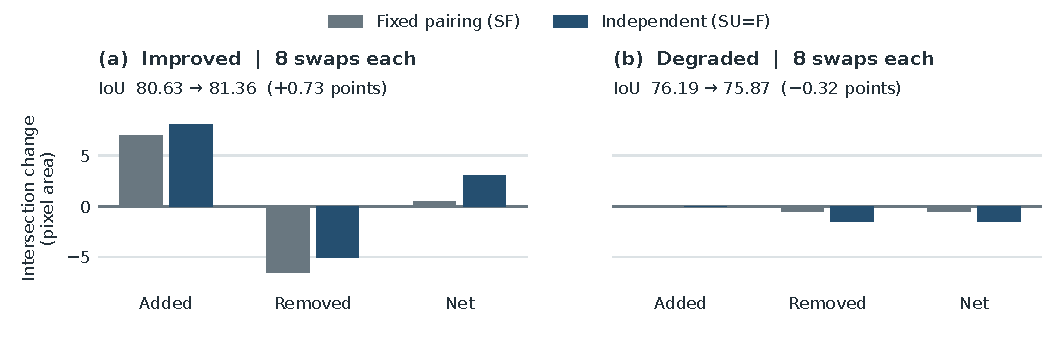
\includegraphics[width=0.83\textwidth]{figures/dev705_overlap_cases.pdf}
\caption{Observed RF-DETR matches on HRSID DEV705, occupancy-head seed 5217. Both policies use eight additions and eight removals. Bars show the reference intersection gained by additions, lost through deletions, and the net change from the native mask. The two cases are nearest the median of the observed IoU differences within each sign. All values use the native cells and the original polygon.}
\label{fig:dev-cases}
\end{figure*}

Fig.~\ref{fig:segrefiner-cases} gives a wider-edit comparison on Instance-RSDD. The published SegRefiner-LR writer~\cite{segrefiner} improves 14 of the 39 eligible reference matches it edits and worsens 25. In the median-sign improvement, the writer trims an extension beyond the hull and raises IoU from 58.68 to 60.96. In the loss case, the write removes reference area at both ends and along a narrow side, lowering IoU from 71.93 to 67.43. The local occupancy writes give 58.89 and 71.95 on these same references. The mixed outcomes are consistent with the signed-loss analysis below. The spatial pooling in the display can break a thin reference contour into segments. The overlap values use the unpooled masks.

\begin{figure*}[!t]
\centering
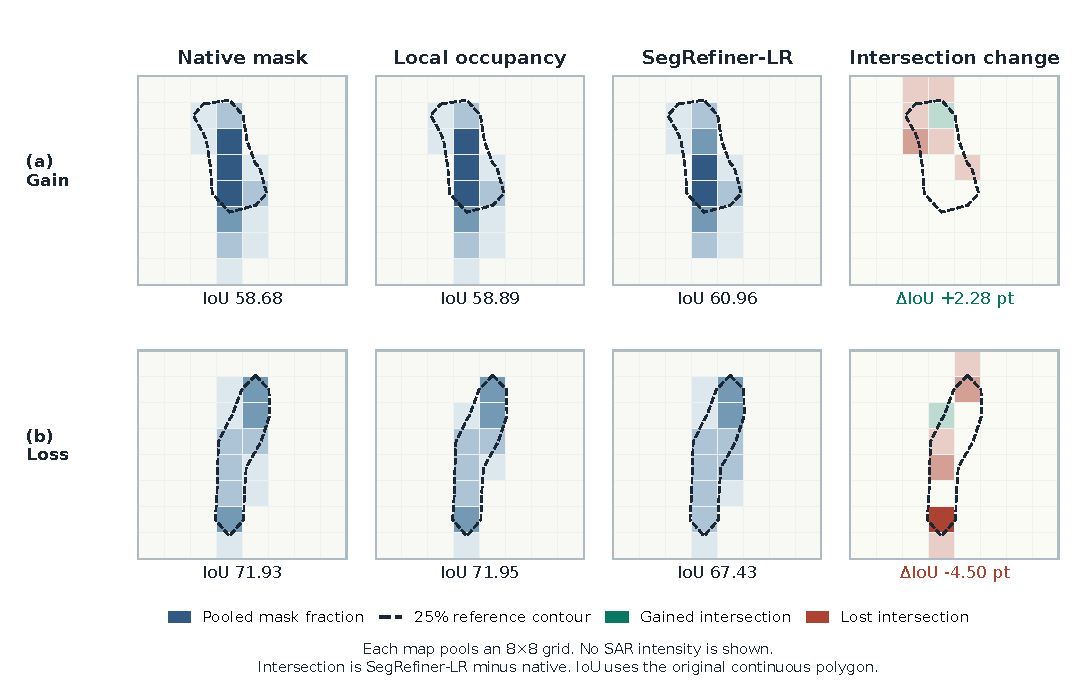
\includegraphics[width=0.87\textwidth]{figures/rsdd74_segrefiner_cases_binned.pdf}
\caption{Observed gain and loss from the original SegRefiner-LR writer on the Instance-RSDD reserve, with the native and local occupancy masks on the same matches. The cases are nearest the within-sign medians among 39 exposed matches. The public panels pool spatial occupancies and intersection changes into an \(8\times8\) grid and display the 25\% reference-occupancy contour. IoU and area changes use the original native raster and author polygon.}
\label{fig:segrefiner-cases}
\end{figure*}

\FloatBarrier
\section{Ablation Studies}
\label{sec:ablation}

\subsection{Independent addition and removal positions}

We combine the addition and removal sites from the fixed-pair and independent writes in a \(2\times2\) comparison. Each hybrid inherits its detector score, writable support, and realized signed counts from the same candidate. On the 74-chip reserve, each arm makes 30,841 exchanges across the complete stream. The factorial comparison therefore isolates the positions chosen on each side of the original mask.

\begin{table*}[t]
\centering
\caption{Mask AP in points for the spatial choice on each side at identical signed counts. Gaofen-3 uses two head fits on the same 583 chips and the same frozen detector. The 42-chip date-separated view is nested within the reserve.}
\label{tab:signed-side-ablation}
\footnotesize
\begin{tabular}{@{}llrrrr@{}}
\toprule
View & Head seed & Both fixed & Independent add & Independent remove & Both independent\\
\midrule
Gaofen-3, 583 chips & 5217 & 61.036 & 61.331 & 61.286 & \textbf{61.518}\\
Gaofen-3, 583 chips & 5218 & 60.984 & 61.207 & 61.302 & \textbf{61.468}\\
Reserve, 74 chips & 5217 & 58.278 & 58.545 & 58.426 & \textbf{58.714}\\
Date-separated, 42 chips & 5217 & 61.283 & 61.769 & 61.698 & \textbf{62.123}\\
\bottomrule
\end{tabular}
\end{table*}

Each single-side change raises mask AP, and freeing both sides gives the highest AP in all four rows of Table~\ref{tab:signed-side-ablation}. On Gaofen-3, independent selection on both sides gains 0.175 continuous-IoU points over independent additions alone (paired 95\% interval \([0.130,0.222]\)) and 0.085 over independent removals alone (\([0.049,0.120]\)). The corresponding gains on the reserve are 0.170 (\([0.108,0.251]\)) and 0.148 (\([0.042,0.252]\)) across 47 eligible matches in 12 parents. The two signed changes are additive in intersection area at a fixed hull. The AP interaction ranges from \(-0.063\) to \(+0.020\) points across the main views, where edited masks can alter matching at each threshold.

\subsection{Ranking, support, and the number of writes}

A geometric ranking remains competitive under the same spatial and count constraints. On the 74-chip reserve, occupancy ranking at the dynamic-attraction budget~\cite{atkinson} gains 0.468 AP and 0.431 continuous-IoU points over dynamic attraction, and 0.203 AP and 0.301 IoU over static attraction. Static attraction leads by 0.173 AP75. Capped PointRend~\cite{pointrend} supplies a learned control on the same endpoints and counts. On Gaofen-3, occupancy improves on it by 0.312 AP and 0.250 fixed-match IoU points. Full RoI PointRend has 0.200 higher AP than the complete-support occupancy writer and 1.744 lower AR100. The full paste changes support and edit counts. These comparisons separate ranking quality from the performance of the complete refinement pipeline.

We also cross the writable support and the flip limit on the same frozen five-iteration Phoenix response~\cite{phoenix}. On the PSeg-SSDD official allocation, imposing the exact count on the whole grid reduces writes from 3,391,327 to 147,540. This raises AP by 2.525 points and fixed-match IoU by 4.001 points (\([2.644,5.382]\)). Applying the count limit on sampled support raises IoU by 0.422 points, so the strongest effect of the limit occurs when the whole grid is writable. Within sampled support, equal signed counts then add 1.842 AP and 1.151 IoU points over the free split at exactly 147,540 flips. Static attraction still leads the balanced Phoenix writer by 0.195 AP at that budget. On the 74-chip reserve, the author LVIS whole-mask policy loses 17.779 AP points relative to same-response matched-count writing. The matched-endpoint Phoenix ranking itself leads occupancy by 0.308 AP, with a paired IoU interval spanning zero.

For SegRefiner-LR, applying the original deletions lowers continuous IoU by 4.092 points relative to native on the 39 exposed Instance-RSDD matches, and by 4.087 relative to retaining the original additions alone. The corresponding losses on 67 exposed PSeg-SSDD matches are 4.03 and 3.98 points. A deletion cap based on the number of additions recovers 0.907 and 0.878 AP points over the original writer. The capped policies trail the addition-only and local occupancy policies on these two evaluated cohorts. Preserving predicted area and preserving the useful part of a proposed update are distinct design choices.

\subsection{Spatial dependence in the allocation score}

We fit a joint model for disjoint four-neighbor endpoint pairs, motivated by the dependence studied in RankSEG-DEP~\cite{rankdep}. The models share endpoint marginals and the same finite signed action menus. Relative to independent predictions of the same pairs, the joint model lowers four-state Brier loss by 0.058 and 0.089 on held FIT groups under the two references. It also improves on coefficients fit after sign-preserving nonspatial rewiring. With frozen coefficients, spatially dependent expected-IoU selection alters 212 of 8,785 positive-budget candidate writes compared with independent expected-IoU selection. Only one of 206 common positive-budget native matches changes. Mask AP is identical under both references. Fixed-match raster IoU changes by zero and 0.00175 points, with the latter paired interval touching zero. This diagnostic supports a local probability-model improvement on the represented FIT groups and a small effect on the tested source decisions.

\section{Discussion and Reproducibility}
\label{sec:discussion}

The reference mask matters most where the editor changes the label. On the same 232 historical SSDD images, the natural-count endpoint policy gains 0.344 AP points over native under PSeg-SSDD and loses 0.491 under SPSD. Under variable signed allocation on SAR-SSP, the two frozen occupancy outputs are checked against the same author raster. Their signed intersection-gain overestimates are 0.896 and 0.628 points of reference area on the selected edits. For that contrast, 392 of the 393 gained false-foreground cells connect to the largest component containing retained fixed-policy foreground. The evidence places the excess chiefly on an attached region. These diagnostics concern selected mask changes under the available annotations.

Proposal coverage further bounds the utility of post-processing. In the frozen RF-DETR SAR-SSP comparison, reference-guided edits within the original support and cap recover just one of 47 unmatched hulls at mask IoU 0.50. Arbitrary replacement within the existing boxes admits nine recoveries at fixed area and a further 19 if area can vary. The latter figures are per-hull ceilings that permit reuse of a candidate. The small UEIKAP positive-budget population~\cite{ueikap} provides another case where few released hulls can benefit from editing. Geometry gains also have limited implications for physical sizing. Measured length-error changes in the common NovaSAR and Sentinel-1 AIS cohorts are uncertain under the paired intervals~\cite{nastar,gulf}.

The two Gaofen-3 detector fits share initialization and evaluation images. The 42-chip date-separated evaluation is nested within the Instance-RSDD reserve. These dependencies bound the transfer interpretation. For the prospective Umbra study, native, local, and Phoenix predictions are frozen on 12 preselected windows. A separate 24-acquisition supplement has completed native readback and frozen local-edit replay. Both await the two independent reference returns and scoring. Each has its own predeclared acquisition-coverage and interval criteria.

On the 74-chip reserve, with detector outputs available, mean single-thread refinement costs are 227.1 ms/image for occupancy writing, 1,221.5 for same-count PointRend, and 1,049.2 for full RoI PointRend. The same-count hybrid still renders the complete RoI. The \href{https://github.com/bingzhi495-creator/SAR-SEAL-research}{project repository} provides configuration, evaluation code, editable figures, and verified aggregate scores. Independent replay reproduced 3,434 tabulated entries on HRSID official and Instance-RSDD test and 1,470 entries on the 74-chip reserve with detector 5202 and head 5217. Exact reproduction requires the designated frozen weights, supplied separately, and the original annotations obtained through the documented dataset providers.


\section{Conclusion}
At the same signed counts, re-pairing and relaxing the inherited displacement cap improve HRSID DEV705 mask AP and continuous overlap. The full Instance-RSDD reserve retains a gain over bounded re-pairing, with greater uncertainty in its 42-chip sensitivity view. One-pixel boundary improvements over distance-first pairing are supported on the reserve and one of the two Gaofen-3 detector fits. At fixed total edits, the variable split improves both SSDD development references across three fits. Frozen SAR-SSP transfer reduces misses while adding excess foreground and leaves the geometry effect uncertain.

\section*{Acknowledgment}
OpenAI Codex assisted with English drafting and editing, schematic and vector-figure preparation, and the experimental analysis code. The method illustrations use worked examples. The quantitative figures and qualitative panels identify their observed data and any spatial aggregation.

\begin{thebibliography}{28}
\bibitem{hrsid} S. Wei, X. Zeng, Q. Qu, M. Wang, H. Su, and J. Shi, ``HRSID: A high-resolution SAR images dataset for ship detection and instance segmentation,'' \emph{IEEE Access}, vol. 8, pp. 120234--120254, \href{https://doi.org/10.1109/ACCESS.2020.3005861}{2020}.
\bibitem{rsdd} X. Yang, Q. Zhang, Q. Dong, Z. Han, X. Luo, and D. Wei, ``Ship instance segmentation based on rotated bounding boxes for SAR images,'' \emph{Remote Sens.}, vol. 15, no. 5, Art. no. 1324, \href{https://doi.org/10.3390/rs15051324}{2023}.
\bibitem{gao2024} F. Gao, X. Han, J. Wang, J. Sun, A. Hussain, and H. Zhou, ``SAR ship instance segmentation with dynamic key points information enhancement,'' \emph{IEEE J. Sel. Topics Appl. Earth Observ. Remote Sens.}, vol. 17, pp. 11365--11385, 2024. \href{https://doi.org/10.1109/JSTARS.2024.3383779}{10.1109/JSTARS.2024.3383779}.
\bibitem{dfine} A. Saakyan and D. Solntsev, ``D-FINE-seg: Object detection and instance segmentation framework with multi-backend deployment,'' \href{https://arxiv.org/abs/2602.23043}{arXiv:2602.23043}, 2026.
\bibitem{rfdetr} I. Robinson, P. Robicheaux, M. Popov, D. Ramanan, and N. Peri, ``RF-DETR: Neural architecture search for real-time detection transformers,'' in \emph{Proc. Int. Conf. Learn. Represent. (ICLR)}, 2026.
\bibitem{ssdd} T. Zhang \emph{et al.}, ``SAR Ship Detection Dataset (SSDD): Official release and comprehensive data analysis,'' \emph{Remote Sens.}, vol. 13, no. 18, Art. no. 3690, 2021. \href{https://doi.org/10.3390/rs13183690}{10.3390/rs13183690}.
\bibitem{drsnet} Q. Zhang and Z. Han, ``DRSNet: Rotated-ROI ship segmentation for SAR images based on dual-scale cross attention,'' \emph{IEEE Geosci. Remote Sens. Lett.}, vol. 21, pp. 1--5, 2024. \href{https://doi.org/10.1109/LGRS.2024.3420251}{10.1109/LGRS.2024.3420251}.
\bibitem{dacf} S. Yang, X. Zhang, W. An, Z. Li, and N. Chen, ``DACF-Net: A dynamic attention and context fusion network with geometry-aware multi-scale refinement for SAR ship instance segmentation,'' \emph{Int. J. Digit. Earth}, vol. 19, no. 2, Art. no. 2696657, 2026. \href{https://doi.org/10.1080/17538947.2026.2696657}{10.1080/17538947.2026.2696657}.
\bibitem{gcie} W. Luo, J. Lan, Y. Zeng, and W. Xiong, ``GCIE-Net: A global and channel information-enhanced network for ship instance segmentation in SAR images,'' \emph{Remote Sens.}, vol. 18, no. 15, Art. no. 2512, 2026. \href{https://doi.org/10.3390/rs18152512}{10.3390/rs18152512}.
\bibitem{gldet} H. Chang, X. Fu, P. Lang, K. Guo, J. Dong, and S. Chang, ``GLDet: Real-time SAR ship detector based on global semantic information enhancement and local gradient information mining,'' \emph{IEEE Trans. Geosci. Remote Sens.}, vol. 63, Art. no. 5209020, 2025. \href{https://doi.org/10.1109/TGRS.2025.3559551}{10.1109/TGRS.2025.3559551}.
\bibitem{dsr} S.-W. He, W. Xiong, and L.-B. Yao, ``SAR ship instance segmentation method in complex scenes jointly driven by differential physical fields and structured graph reasoning,'' \emph{Acta Electronica Sinica}, pp. 1--11, 2026. \href{https://doi.org/10.12263/DZXB.20260699}{10.12263/DZXB.20260699}.
\bibitem{atkinson} P. M. Atkinson, ``Sub-pixel target mapping from soft-classified, remotely sensed imagery,'' \emph{Photogramm. Eng. Remote Sens.}, vol. 71, no. 7, pp. 839--846, 2005. \href{https://doi.org/10.14358/PERS.71.7.839}{10.14358/PERS.71.7.839}.
\bibitem{xu} Y. Xu and B. Huang, ``A spatio-temporal pixel-swapping algorithm for subpixel land cover mapping,'' \emph{IEEE Geosci. Remote Sens. Lett.}, vol. 11, no. 2, pp. 474--478, 2014. \href{https://doi.org/10.1109/LGRS.2013.2268153}{10.1109/LGRS.2013.2268153}.
\bibitem{rankseg} B. Dai and C. Li, ``RankSEG: A consistent ranking-based framework for segmentation,'' \emph{J. Mach. Learn. Res.}, vol. 24, no. 224, pp. 1--50, \href{https://www.jmlr.org/papers/v24/22-0712.html}{2023}.
\bibitem{rankrma} Z. Wang and B. Dai, RankSEG-RMA: An efficient segmentation algorithm via reciprocal moment approximation, in \emph{Adv. Neural Inf. Process. Syst.}, vol. 38, 2025. \href{https://doi.org/10.52202/085713-5452}{10.52202/085713-5452}.
\bibitem{rankdep} Z. Wang and B. Dai, ``On the relaxation of conditional independence assumption for image segmentation,'' \href{https://arxiv.org/abs/2609.38930}{arXiv:2609.38930}, 2026.
\bibitem{pointrend} A. Kirillov, Y. Wu, K. He, and R. Girshick, ``PointRend: Image segmentation as rendering,'' in \emph{Proc. IEEE/CVF Conf. Comput. Vis. Pattern Recognit. (CVPR)}, 2020, pp. 9799--9808.
\bibitem{segfix} Y. Yuan, J. Xie, X. Chen, and J. Wang, ``SegFix: Model-agnostic boundary refinement for segmentation,'' in \emph{Proc. Eur. Conf. Comput. Vis. (ECCV)}, 2020, pp. 489--506.
\bibitem{bpr} C. Tang, H. Chen, X. Li, J. Li, Z. Zhang, and X. Hu, ``Look closer to segment better: Boundary patch refinement for instance segmentation,'' in \emph{Proc. IEEE/CVF Conf. Comput. Vis. Pattern Recognit. (CVPR)}, 2021, pp. 13926--13935.
\bibitem{refinemask} G. Zhang, X. Lu, J. Tan, J. Li, Z. Zhang, Q. Li, and X. Hu, ``RefineMask: Towards high-quality instance segmentation with fine-grained features,'' in \emph{Proc. IEEE/CVF Conf. Comput. Vis. Pattern Recognit. (CVPR)}, 2021, pp. 6861--6869.
\bibitem{phoenix} B. Kim and S. J. Hwang, ``Learning from adversity: Semantic-aware mask refinement through adversarial perturbation,'' in \emph{Proc. Eur. Conf. Comput. Vis. (ECCV)}, 2026, pp. 75--92. \href{https://doi.org/10.1007/978-3-032-37520-9_5}{10.1007/978-3-032-37520-9\_5}.
\bibitem{segrefiner} M. Wang, H. Ding, J. H. Liew, J. Liu, Y. Zhao, and Y. Wei, ``SegRefiner: Towards model-agnostic segmentation refinement with discrete diffusion process,'' in \emph{Adv. Neural Inf. Process. Syst.}, vol. 36, 2023. \href{https://proceedings.neurips.cc/paper_files/paper/2023/hash/fc0cc55dca3d791c4a0bb2d8ddeefe4f-Abstract-Conference.html}{Proceedings}.
\bibitem{slgsea} R. Deng, T. Zhang, G. Gao, L. Zhang, S. Wei, and X. Zhang, ``SLGSea: Spatialized language guidance with scattering-aware query construction for ship--sea--land panoptic segmentation in SAR imagery,'' project repository and dataset release. \href{https://github.com/deng1218/SLGSea}{Code and data}.
\bibitem{airsarship} X. Sun, Z. Wang, Y. Sun, W. Diao, Y. Zhang, and K. Fu, ``AIR-SARShip-1.0: High-resolution SAR ship detection dataset,'' \emph{J. Radars}, vol. 8, no. 6, pp. 852--862, 2019. \href{https://doi.org/10.12000/JR19097}{10.12000/JR19097}.
\bibitem{boundaryiou} B. Cheng, R. Girshick, P. Doll{\'a}r, A. C. Berg, and A. Kirillov, ``Boundary IoU: Improving object-centric image segmentation evaluation,'' in \emph{Proc. IEEE/CVF Conf. Comput. Vis. Pattern Recognit. (CVPR)}, 2021. \href{https://arxiv.org/abs/2103.16562}{arXiv:2103.16562}.
\bibitem{ueikap} A. Mazzeo \emph{et al.}, ``UEIKAP dataset,'' Zenodo, ver. 1.0, \href{https://doi.org/10.5281/zenodo.18391027}{2026}.
\bibitem{nastar} B. Hosseiny, K. Kamirul, O. Pappas, and A. Achim, ``NASTaR: A NovaSAR-based automated ship target recognition dataset,'' \emph{IEEE Geosci. Remote Sens. Lett.}, vol. 23, Art. no. 1502605, 2026. \href{https://doi.org/10.1109/LGRS.2026.3679941}{10.1109/LGRS.2026.3679941}.
\bibitem{gulf} M. Shaya, ``SAR Ship Gulf: Sentinel-1 GRD ship chips with AIS labels,'' Zenodo, ver. 1, 2026. \href{https://doi.org/10.5281/zenodo.21000650}{10.5281/zenodo.21000650}.
\end{thebibliography}

\end{document}
